\section{Ziel des Versuchs}
\label{sec:Ziel des Versuchs}
Die Funktionsweise eines Lock-In-Verstärkers soll kennengelernt und überprüft werden.
\section{Theorie}
\label{sec:Theorie}
\subsection{Lock-In-Verstärker}
    Ein Lock-In-Verstärker wird vorallem zur genauen Messung von verrauschten Signalen verwendet.
    Dazu wird ein Messsignal durch ein Referenzfrequenz $\omega_0$ moduliert, anschließend wird das
    hierzugehörige Nutzsignal $U_\text{sig}$ durch einen Bandpassfilter von Rauschanteilen mit höheren und niedrigeren Frequenzen
    befreit. Danach wird das Signal, wie auch in Abbildung \ref{fig:funktion} zu sehen, mit einem Referenzsignal
    $U_\text{ref}$, welches dieselbe Frequenz $\omega_0$ wie $U_\text{sig}$ hat, multipliziert. Die Phase $\Phi$ der Referenzspannung im Vergleich zu $U_sig$
    ist dabei durch einen Phasenschieber veränderlich. 
    Für eine zu messende Sinusspannung, wie im Versuch, gilt also
    \begin{equation}
        U_\text{sig} = U_0 sin(\omega t)
    \end{equation} 
    \begin{equation}
        U_\text{ref} = \frac {4}{\pi} (\sin (\omega t) + \frac {1}{3} \sin(3 \omega t) + ... )
    \end{equation}
    wobei $U_\text{ref}$ durch ein Rechtecksignal moduliert wird. Das gemischte Signal ergiebt somit
    \begin{equation}
        U_\text{sig} \times U_\text{ref} = \frac {2}{\pi} U_0 (1- \frac{2}{3} \cos (2 \omega t) - \frac {2}{15} \cos (4 \omega t) - ...).
    \end{equation}
    Das resultierende Signal $U_\text{sig} \times U_\text{ref}$ wird anschließend durch einen Tiefpaß über ein Vielfaches der Periodenlänge
    integriert, was dazu führt, dass die Oberfrequenzen $\omega$ des Mischsignals unterdrückt werden. Das Ausgangssingnal ist dann
    \begin{equation}
    \label{eqn:u_out}
        U_\text{out} = \frac{2}{\pi} U_0 \cos (\Phi) .
    \end{equation}
    Indem nun $\Delta \Phi = 0$ gewählt wird, werden das Eingangs- und das Referenzsignal synchronisiert, so dass sich Gleichung \ref{eqn:u_out}
    zu
    \begin{equation}
        U_\text{out} = \frac{2}{\pi} U_0
    \end{equation}
    vereinfacht. Der Tiefpassfilter kann dabei eine fast beliebig kleine Bandbreite $\Delta \nu  = \frac{1}{\pi R C}$ haben, da sich die Zeitkonstante $\Tau = R C$ sehr groß wählen lässt.
    Hierdurch sind Güten mit bis zu $Q = 100000$ möglich.
    \begin{figure*}[!h]
        \centering
        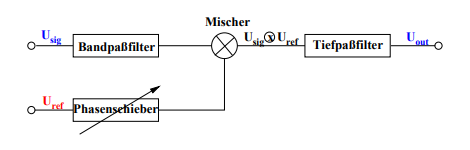
\includegraphics{content/abbildung1.png}
        \caption{Funktionsweise eines Lock-In-Verstärkers \cite[1]{V303}}
        \label{fig:funktion}
        \end{figure*}
        \newpage
\subsection{Photodiode}
    Bei der Photodiode handelt es sich um eine p-n-Diode, welche an einem p-n-Übergang eintreffende Photonen in elektrischen Strom umwandeln. 
    Der Effekt der dabei in der Diode stattfindet nennt sich Photoeffekt. Dabei bewirken die Photonen 
    in der Sperrschicht ein Elektron-Loch-Paar. Da es sich hierbei um einen Halbleiter handelt, werden die Elektronen zur n-Seite und die Löcher zur p-Seite beschleunigt.
    Hierdurch kommt es zur Erhöhung der Elektrischen Feldstärke am Übergang, was schlussendlich einen elektrischen Strom bewirkt. \cite{diode}